\begin{figure}[h!]
    \centering
    \caption{Effects of \emph{Plan Cuadrante} on Police Clearance}
    \label{fig:arrests_reportedcrime}
    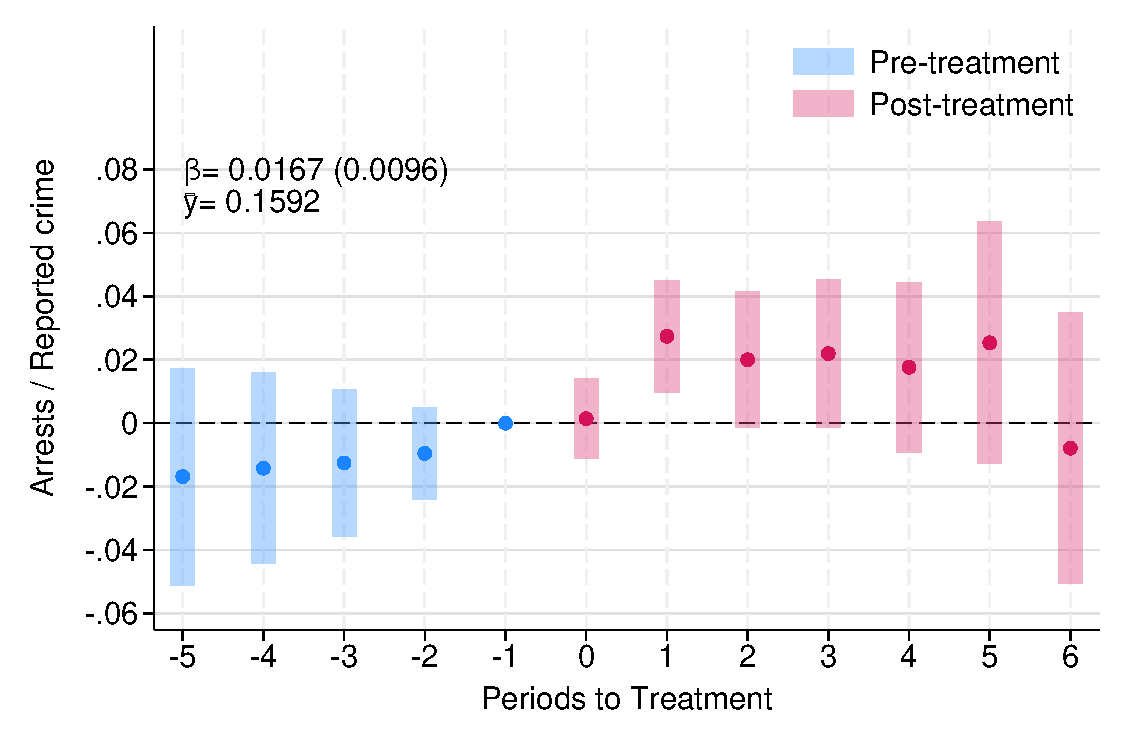
\includegraphics[width=0.7\textwidth]{../manuscript/Graphs/arrests_over_reportedcrime_allcomunas.pdf}
    \begin{minipage}{\textwidth}
    \footnotesize
   Notes: This figure shows the dynamic effects of the \emph{Plan Cuadrante} on the ratio of arrests to reported crime. This outcome captures the share of reported offenses that result in an arrest, and can therefore be interpreted as a measure of police clearance or apprehension effectiveness: higher values indicate that a larger fraction of crimes brought to the attention of the police is followed by an arrest. The estimation is conducted using the procedure developed in \citet{Callaway} for difference-in-differences with staggered treatment adoption. The dots in the figure represent the estimated coefficients and the bars behind them 95\% confidence intervals. Standard errors are clustered at the municipality level using the wild bootstrapping procedure. The pooled effect and the mean outcome before the introduction of the treatment---computed as in Figure \ref{fig:figure02}, using only the pre-treatment observations of treated units---are also presented in the panel.
    \end{minipage}
\end{figure}
